% ------------------------------------------------------------------------------
% 	Dokumentenklasse
% ------------------------------------------------------------------------------

% Dokumentenklasse: scrreport (KoMa Script Dokumente sind für deutsche Dokumente optimiert)
% Dokumentenklasse Optionen: 
%	12pt 			--> 12pt Schriftgröße
%	a4paper 		--> DINA4 Papierformat
%	parskip 		--> Absätze mit Freizeilen statt Einzügen kennzeichnen
%	listof=totoc 	--> Abbildungs- und Tabellenverzeichnis in Inhaltsverzeichnis aufnehmen
%	bitotoc			--> Literaturverzeichnis in Inhaltsverzeichnis aufnehmen
\documentclass[12pt, a4paper, parskip, listof=totoc, bibtotoc]{scrreprt}

% ------------------------------------------------------------------------------
%	Wichtige Pakete
% ------------------------------------------------------------------------------

% geometry 	--> Seitenränder einstellen
\usepackage[left=3cm, right=3cm, top=2cm, bottom=2cm, includehead=true, includefoot=true]{geometry}

% setspace	--> Zeilenabstand auf eineinhalb setzen
\usepackage[onehalfspacing]{setspace}

% inputenc 	-->	direkte Eingabe von Umlauten mit [utf8]
\usepackage[utf8]{inputenc}

% fontenc	--> Darstellung von Umlauten mit [T1] 
\usepackage[T1]{fontenc}

% babel 	--> Neue deutsche Rechtschreibung mit [ngerman]
\usepackage[ngerman]{babel}

% amsmath 	--> Erweiterung für Latex-Mathe
\usepackage{amsmath}

% amssymb 	--> Zusätzliche Mathesymbole
\usepackage{amssymb}

% graphicx 	--> Bilder einbinden
\usepackage{graphicx}

% url 		--> URLs einfügen
\usepackage{url}

% pdfpages 	--> Einbinden von externen PDFs
\usepackage{pdfpages}

% hyperref 	--> PDF Verlinkungen im Inhaltsverzeichnis
\usepackage{hyperref}

% acronym 	--> Abkürzungsverzeichnis
\usepackage{acronym}

% caption 	--> Bildunterschriften
\usepackage{caption}
\usepackage{subcaption}

% tabularx 	--> Verbesserte Tabellen
\usepackage{tabularx}

% booktabs 	--> Schönere Tabellen
\usepackage{booktabs}

% fancyhdr 	--> Schöne Kopf- und Fußzeilen
\usepackage{fancyhdr}

% pgffor 	--> Foreach-Loops
\usepackage{pgffor}

% float 	--> Positionierung
\usepackage{float}

% blindtext	--> Blindtext generieren
\usepackage{blindtext}

% ------------------------------------------------------------------------------
%	Kopf- und Fußzeile konfigurieren
% ------------------------------------------------------------------------------

\pagestyle{fancy}

\lhead{\textsc{\rightmark}}
\chead{}
\rhead{\textsc{\leftmark}}

\lfoot{}
\cfoot{\thepage}
\rfoot{}

% ------------------------------------------------------------------------------
%	Allgemeine Informationen (Ändern!!!)
% ------------------------------------------------------------------------------

\def\arbeitstyp{Bachelorarbeit}

\def\titel{Hier könnte Ihr Titel stehen}

\def\autor{Max Mustermann}
\def\strasse{Musterstraße}
\def\hausnummer{1}
\def\plz{12345}
\def\ort{Musterort}

\def\gutachter{Dr. Maria Musterfrau}

\def\ausbildungsbetrieb{Musterfirma GmbH}
\def\ausbildungsplz{12345}
\def\ausbildungsort{Musterort}

\def\semester{2999/6}

\def\abgabedatum{31.12.2999}

\def\betrieblicherbetreuer{Franz Kanz}

\def\wortanzahl{15.000}

% ------------------------------------------------------------------------------
%	Zusätzliche Konfiguration (Ändern!!!)
% ------------------------------------------------------------------------------
% Will man die folgenden Komponenten in seiner Arbeit haben oder nicht, bitte den entsprechenden Wert auf true oder false setzen.

% Sperrvermerk
\newif\ifsperrvermerk
\setboolean{sperrvermerk}{true}

% Vorwort
\newif\ifvorwort
\setboolean{vorwort}{true}

% Abkürzungsverzeichnis
\newif\ifabkuerzungsverzeichnis
\setboolean{abkuerzungsverzeichnis}{true}

% Gleichgeschlechtlichkeitsdisclaimer unter dem Inhaltsverzeichnis
\newif\ifgleichgeschlechtlichkeitsdisclaimer
\setboolean{gleichgeschlechtlichkeitsdisclaimer}{true}

% Logos auf Titelblatt
\newif\iflogosauftitelblatt
\setboolean{logosauftitelblatt}{false}

% ------------------------------------------------------------------------------
%	Beginn des Dokuments
% ------------------------------------------------------------------------------

\begin{document}
	
%	Titelblatt
	\thispagestyle{empty}
\begin{center}
	
	\iflogosauftitelblatt
		\begin{figure}[h]
			\begin{subfigure}{0.5\textwidth}
				\centering
				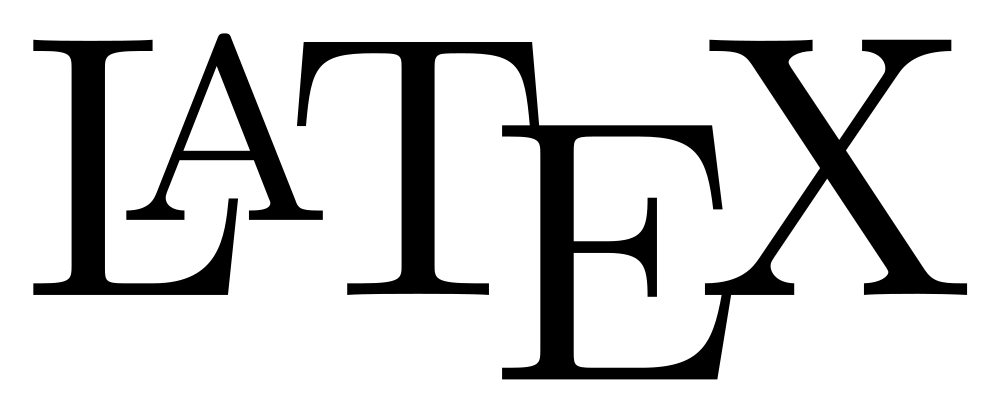
\includegraphics[width=4cm, keepaspectratio]{./logos/unternehmen.png}
			\end{subfigure}
			\begin{subfigure}{0.5\textwidth}
				\centering
				
\includegraphics[width=4cm, keepaspectratio]{./logos/dhbw.png}
			\end{subfigure}
		\end{figure}
	\fi

	\vspace*{\fill}
	
	\textbf{\large \titel}
	
	\vspace{\fill}
	
	\textbf{\arbeitstyp}
	
	an der Dualen Hochschule Baden-Württemberg Heidenheim in der Fakultät Wirtschaft im Studiengang Wirtschaftsinformatik \\
	
	\vspace{\fill}
	
	eingereicht von
		
	\autor \\
	\strasse{} \hausnummer \\
	\plz{} \ort \\
	
	\vspace{\fill}
	
	\begin{table}[b]
		\centering
		\begin{tabularx}{10cm}{lX}
			Gutachter: & \gutachter \\
			Ausbildungsbetrieb: & \ausbildungsbetrieb \newline \ausbildungsplz{} \ausbildungsort \\
			Semester: & \semester \\
			Abgabedatum: & \abgabedatum \\
			Betrieblicher Betreuer: & \betrieblicherbetreuer \\
		\end{tabularx}
	\end{table}
	
\end{center}
	
%	Römische Seitenzahlen
	\pagenumbering{Roman}
	
%	Sperrvermerk
	\ifsperrvermerk \chapter*{Sperrvermerk}
Die vorliegende \arbeitstyp{} enthält vertrauliche Daten und Informationen der \ausbildungsbetrieb. Veröffentlichungen oder Vervielfältigungen - auch nur auszugsweise - sind ohne ausdrückliche schriftliche Genehmigung der Unternehmen nicht gestattet. Die \arbeitstyp{} ist ausschließlich den Korrektoren sowie den Mitgliedern des Prüfungsausschusses zugänglich zu machen. \fi
	
%	Vorwort
	\ifvorwort \chapter*{Vorwort}
Hier könnte Ihr Vorwort stehen. \fi
	
%	Abstract
	\include{./standardkomponenten/abstract}
	
%	Inhaltsverzeichnis
	\tableofcontents
	\ifgleichgeschlechtlichkeitsdisclaimer Aus Gründen der besseren Lesbarkeit wird auf die gleichzeitige Verwendung weiblicher und männlicher Sprachformen verzichtet.

Sämtliche Personenbezeichnungen gelten gleichwohl für beiderlei Geschlecht. \fi
	
%	Abkürzungsverzeichnis
	\ifabkuerzungsverzeichnis \chapter*{Abkürzungsverzeichnis}
\addcontentsline{toc}{chapter}{Abkürzungsverzeichnis}
\begin{acronym}
	\acro{SQL}{Structured Query Language}
\end{acronym} \fi
	
%	Abbildungsverzeichnis
	\listoffigures
	\cleardoublepage
	
%	Tabellenverzeichnis
	\listoftables
	\cleardoublepage
	
% 	Arabische Seitenzahlen
	\pagenumbering{arabic}
	
%	Inhalt
	\foreach \i in {00, 01, 02, 03, 04, 05, 06, 07, 08, 09, 10, ...,99} {%
		\edef\FileName{./kapitel/\i .tex}%     
		\IfFileExists{\FileName}{%
			\input{\FileName}%       
		}
	}

%	Literaturverzeichnis
%	bibliographystyle 	--> einer von [plain, abbrv, alpha, abstract, apa, unsrt]
	\bibliographystyle{plain}
%	bibliography 		--> Pfad zur Bibtex-Datei (ohne .bib am Ende)
	\bibliography{./literatur/bibfile}
	
% 	Anhang
	\appendix
\chapter{Erster Anhang}
\begin{figure}[H]
	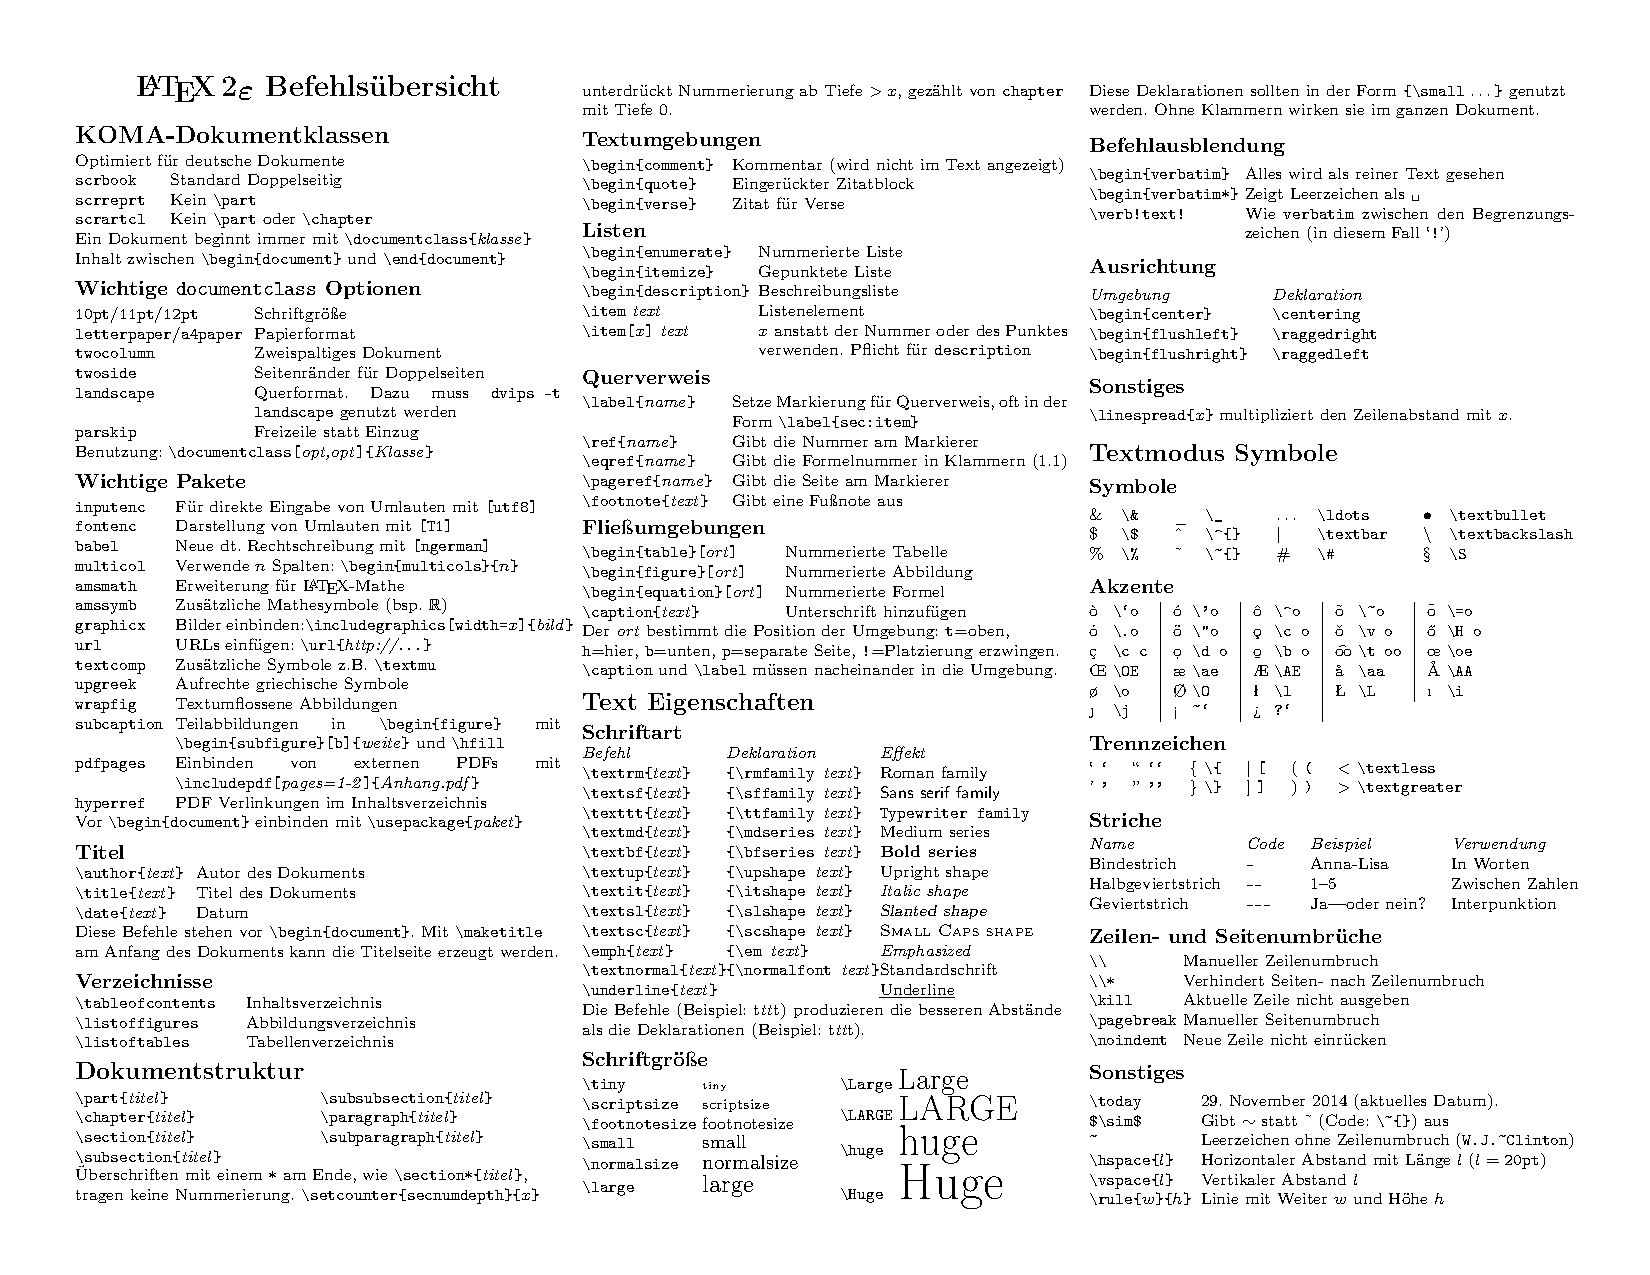
\includegraphics[width=\textwidth, keepaspectratio]{latexsheet-de}
	\caption*{\LaTeX{} Cheatsheet}
	\label{latexsheet}
\end{figure}

\chapter{Zweiter Anhang}
\blindtext
	\cleardoublepage

%	Ehrenwörtliche Erklärung
	\thispagestyle{empty}
\chapter*{Ehrenwörtliche Erklärung}
Ich versichere hiermit, dass ich meine \arbeitstyp{} mit
dem Titel \begin{quote}\textit{\titel}\end{quote} selbständig verfasst und keine anderen als die angegebenen Quellen und erlaubten Hilfsmittel benutzt habe. Alle wörtlichen Zitate in der Arbeit wurden durch Anführungszeichen eindeutig gekennzeichnet. Die Arbeit wurde in gleicher oder ähnlicher Form bei keiner anderen Prüfung vorgelegt. 

Der Textteil der Arbeit umfasst \wortanzahl{} Wörter. 
\begin{figure}[h]
	\centering
	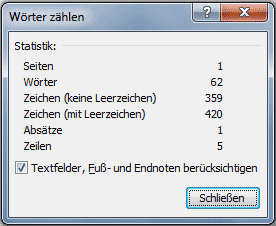
\includegraphics[width=5cm, keepaspectratio]{./bilder/wortanzahl.png}
	\caption*{Wortanzahl der Arbeit}
\end{figure}

\ort, \today \\

\begin{tabular}{@{}l@{}}\hline
	\autor
\end{tabular}
	
\end{document}